\section{Muhammad Reza Syachrani(1174084)}
\subsection{Instalasi Map Server}
\begin{enumerate}
    \item Download aplikasi ms4w melalui website ms4w.com/download.html
    \hfill\break
    \begin{figure}[H]
		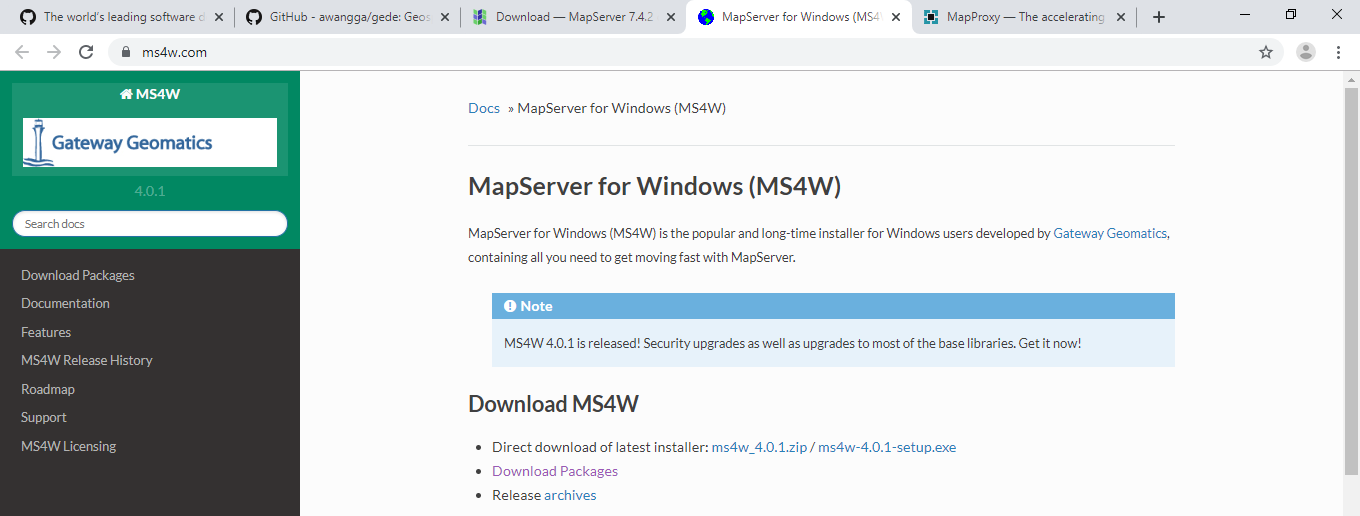
\includegraphics[width=4cm]{figures/tugas4/1174084/1.png}
		\centering
		\caption{Download MS4W}
    \end{figure}
    \hfill\break

    \item Setelah download buka aplikasi untuk melakukan instalasi.
    \item Pada saat instalasi pilih Full Install
\end{enumerate}

\subsection{Konfigurasi Map Server}
Ketika instalasi selesai, lakukan konfigurasi
\begin{enumerate}
  \item Buka folder ms4w pada c:/ms4w. Lalu masuk ke folder apache
  \hfill\break
    \begin{figure}[H]
		
\includegraphics[width=4cm]{figures/tugas4/1174084/3.png}
		\centering
		\caption{Folder Apache}
    \end{figure}


  \item Masuk ke folder conf
  \hfill\break
    \begin{figure}[H]
		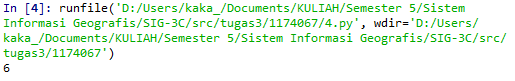
\includegraphics[width=4cm]{figures/tugas4/1174084/4.png}
		\centering
		\caption{Folder conf}
    \end{figure}

  \item Buka file httpd.conf menggunakan editor lalu cari tulisan Listen. Karena pada komputer saya port 80 digunakan oleh xampp maka saya ubah.
  \hfill\break
    \begin{figure}[H]
		
\includegraphics[width=4cm]{figures/tugas4/1174084/5.png}
		\centering
		\caption{File httpd.conf}
    \end{figure}

  \hfill\break
    \begin{figure}[H]
		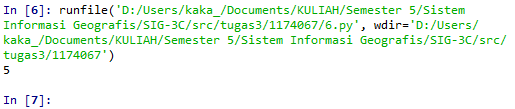
\includegraphics[width=4cm]{figures/tugas4/1174084/6.png}
		\centering
		\caption{Edit file httpd.conf}
    \end{figure}

  \item Kemudian kita restart service milik ms4w dengan cara, membuka windows + r lalu ketik services.msc
  \hfill\break
    \begin{figure}[H]
		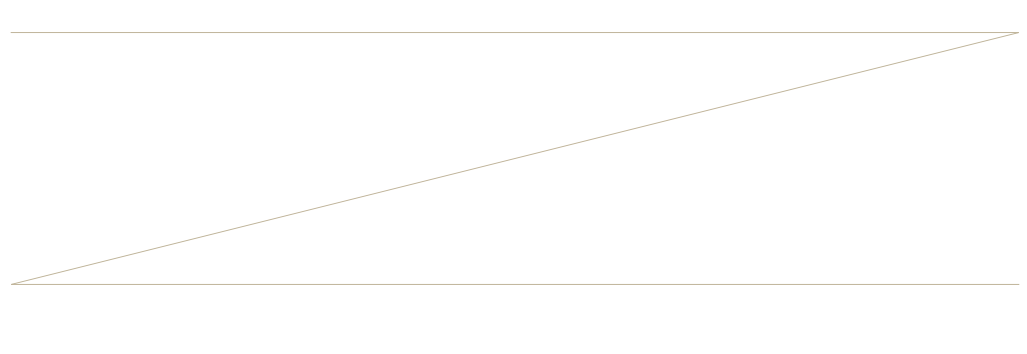
\includegraphics[width=4cm]{figures/tugas4/1174084/7.png}
		\centering
		\caption{Services.msc}
    \end{figure}
    
  \item Cari ApacheMS4WWebServer
  \hfill\break
  \begin{figure}[H]
  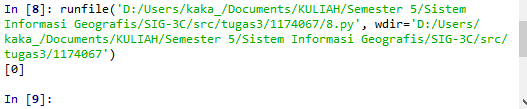
\includegraphics[width=4cm]{figures/tugas4/1174084/8.png}
  \centering
  \caption{pilih ApacheMS4WWebServer}
  \end{figure}

  \item Klik kanan lalu tekan Restart
  \hfill\break
    \begin{figure}[H]
		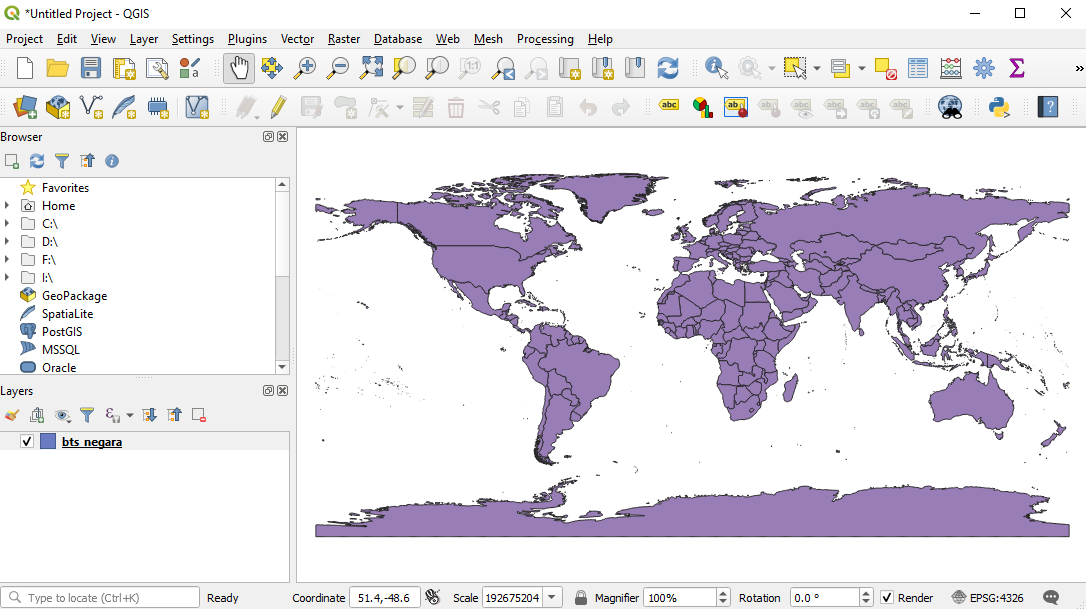
\includegraphics[width=4cm]{figures/tugas4/1174084/9.png}
		\centering
		\caption{Mengakses Halaman Service}
    \end{figure}
\end{enumerate}

\subsection{Instalasi MapProxy}
\begin{enumerate}
  \item Buka Command Prompt pada Windows
  \item Lalu ketikkan pip install MapProxy
  \hfill\break
  \begin{figure}[H]
  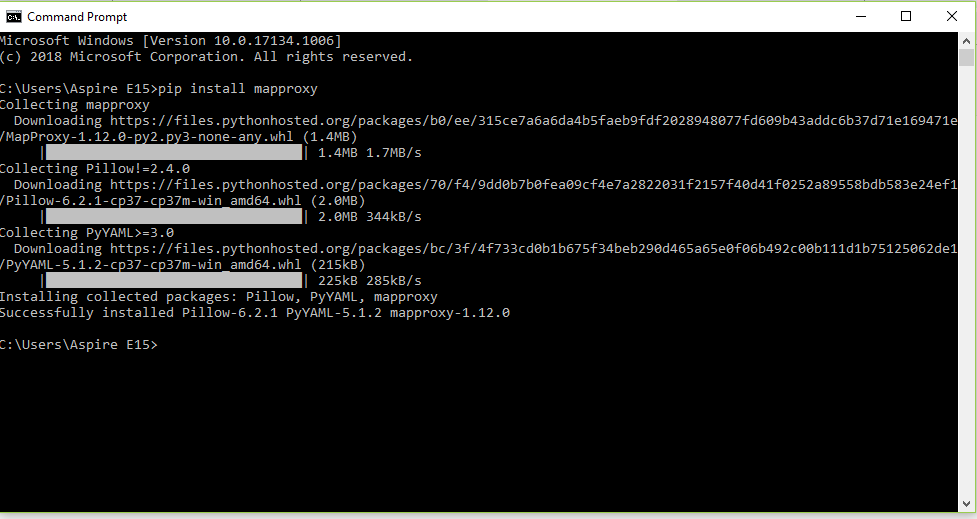
\includegraphics[width=4cm]{figures/tugas4/1174084/10.png}
  \centering
  \caption{Instalasi MapProxy}
  \end{figure}
\end{enumerate}

\subsection{Membuka map menggunakan MapProxy}
\begin{enumerate}
  \item Download / clone git terlebih dahulu file dari https://github.com/awangga/gede
  \item Pastikan path menuju folder gede tidak ada spasi 
  \hfill\break
  
  \item Pada folder gede-master buat folder bernama tmp
  \hfill\break
  \begin{figure}[H]
  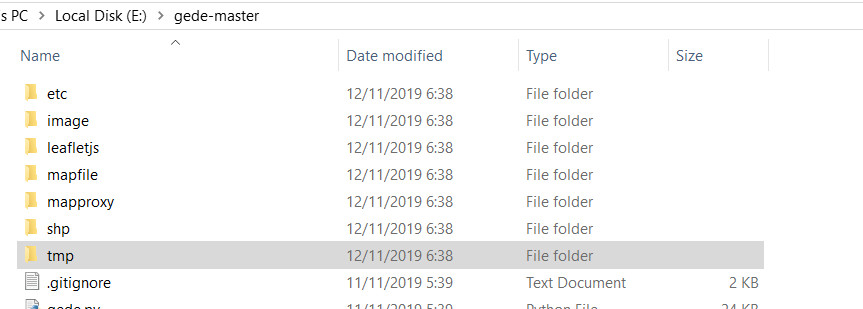
\includegraphics[width=4cm]{figures/Tugas4/1174084/11.png}
  \centering
  \caption{buat folder tmp}
  \end{figure}
 
  \item Setelah itu buka folder mapproxy lalu edit file agm.yaml menggunakan text editor contoh visual code studio
  \item Pada bagian sources lalu ada map:, masukkan pathnya sesuai dengan tempat menyimpan data clone tdi contohnya E:/gede/mapfile/mywms.map
  \hfill\break
  \begin{figure}[H]
  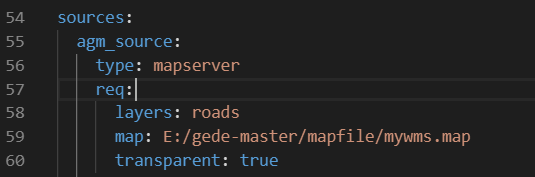
\includegraphics[width=4cm]{figures/Tugas4/1174084/12.png}
  \centering
  \caption{Edit lokasi mymap.map}
  \end{figure}


  \item Kemudian pada bagian binary masukkan lokasi instalasi ms4w yagn berada pada C:/ms4w/Apache/cgi-bin/mapserv.exe
  \item Selanjutnya pada bagian working-dir masukkan path folder temp yang telah kita buat tadi, yang saya E:/gede/tmp
  \hfill\break
  \begin{figure}[H]
  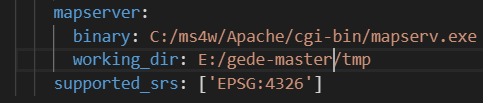
\includegraphics[width=4cm]{figures/Tugas4/1174084/13.png}
  \centering
  \caption{Edit binary dan path working-dir}
  \end{figure}

  \item Setelah itu buka aplikasi MS4W-Shell
  \item Kemudian masuk directory mapproxy pada folder clone tadi ,setelah masuk ke directorinya ketikkan "mapproxy-util serve-develop agm.yaml" pada ms4w-Shell untuk membuka aplikasi mapproxy
  \hfill\break
  \begin{figure}[H]
  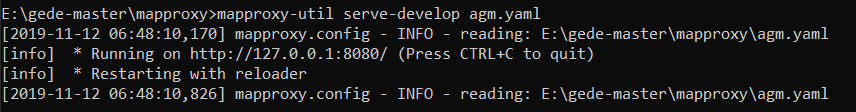
\includegraphics[width=4cm]{figures/Tugas4/1174084/14.png}
  \centering
  \caption{Buka aplikasi mapproxy}
  \end{figure}

  \item Buka browser lalu ketikkan 127.0.0.1:8080
  \hfill\break
  \begin{figure}[H]
  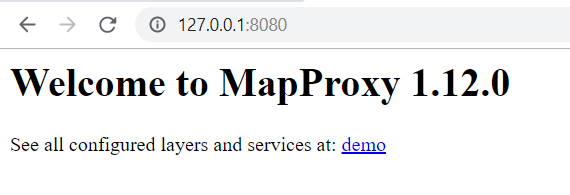
\includegraphics[width=4cm]{figures/Tugas4/1174084/15.png}
  \centering
  \caption{Buka mapproxy pada browser}
  \end{figure}

  \item lalu klik demo untuk melihat map
  \item lalu klik png pada agm, maka mapproxy akan menampilkan map
  \hfill\break
  \begin{figure}[H]
  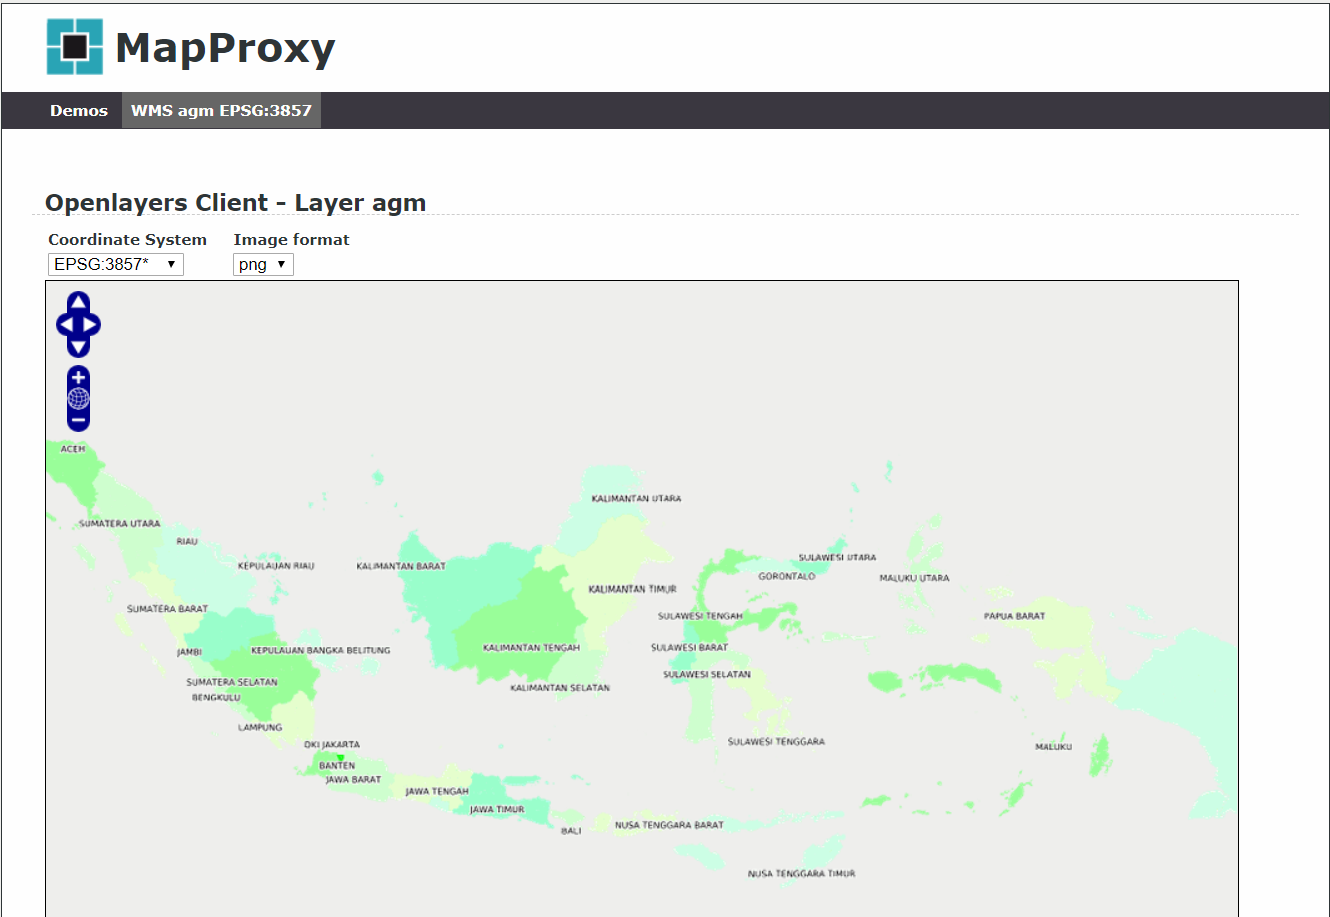
\includegraphics[width=4cm]{figures/Tugas4/1174084/16.png}
  \centering
  \caption{MapProxy menampilkan map}
  \end{figure}

\end{enumerate}

\subsection{Link Youtube}
https://youtu.be/Wjt4Tdz-QNQ